\documentclass[a4paper]{report}
\usepackage{amsmath,amssymb,booktabs,bm,caption,enumerate,float,geometry,graphicx,indentfirst,makecell,multirow,setspace,titlesec}
\geometry{left=4.5cm,right=4.5cm,top=4cm,bottom=4cm}
\captionsetup[figure]{labelsep=period}
\captionsetup[table]{labelsep=period}
\begin{document}
	\renewcommand\thesection{\arabic{section}}
	\begin{Large}
		\begin{center}
			\setlength{\baselineskip}{14pt}
			\vspace{1.25cm}
			\rule[0cm]{11.2cm}{0.03em}\\
			\vspace{0.5cm}
			\textsc{UM-SJTU Joint Institute}\\
			\vspace{0.25cm}
			\textsc{Intro to circuits\\(VE215)}
			\vspace{0.3cm}
			\rule[0cm]{11.8cm}{0.05em}
			\vspace{4.9cm}\\
			\textsc{Laboratory Report}
		\end{center}
	\end{Large}
	\vspace{0.85cm}
	\begin{large}
		\begin{center}
			\textsc{Lab 3}
			\vspace{1em}\\
			\textsc{Transient Lab}
		\end{center}
		\vspace{6cm}
	\end{large}
	\begin{tabular}{l l}
	Name: Yihua Liu&ID: 518021910998\\
	Name: Han Fang&ID: 518370910009\\
	Name: Yiteng Cai&ID: 518370910007\\
	&\\
	Date: \today&\\
	\end{tabular}
	\thispagestyle{empty}
	\newpage
	\section{Introduction}
	\subsection{Objectives}
	\begin{enumerate}[i.]
		\item Apply the theory we learned on the step responses in first- and second-order circuits to series $RC$ and $RLC$ circuits, which we will build in the lab.
		\item Build a series $RC$ circuit, observe its responses to input square wave signal of varied frequency, and explain them based on the theory we learned:
		\begin{itemize}
			\item Relate the observed capacitor voltage and resistor voltage as functions of time to your pre-lab calculations
			\item Explain the changes of both output waveforms in response to the increase of the frequency of the input square wave signal
			\item Explain the amplitudes of the capacitor voltage and the resistor voltage related to the amplitude of the input square wave
		\end{itemize}
		\item Build a series $RLC$ circuit, observe the three types of its responses to input square wave signal, and relate them to the theory you have learned. For the under-damped/ over-damped/ critical damped response, compare the resistance in the circuit measured in the lab with the critical resistance you calculated in the pre-lab.
		\item Build the simplest second-order circuit, an $LC$ tank, and observe oscillations.
	\end{enumerate}
	\subsection{Apparatus \& Theoretical Background}
	Theoretically, the transient responses in electric circuits are described by differential equations. The circuits, whose responses obey the first-order differential equation.
	\begin{equation*}
		\dfrac{\mathrm{d}x(t)}{\mathrm{d}t}+\dfrac{1}{\tau}\cdot x(t)=f(t)
	\end{equation*}
	are called first-order circuits. Their responses are always monotonic and appear in the form of exponential function
	\begin{equation*}
		x(t)=K_1\cdot e^{-(\frac{t}{\tau})}+K_2
	\end{equation*}
	
	A first-order circuit includes the effective resistance $R$ and one energy-storage element, an inductor $L$ or a capacitor $C$.
	
	In an $RC$ circuit, the time constant is
	\begin{equation*}
		\tau=RC.
	\end{equation*}
	
	In an $LC$ circuit, the time constant is
	\begin{equation*}
		\tau=\dfrac{L}{R}.
	\end{equation*}
	
	The fall time of a signal is defined as the interval between the moment when the signal reaches its 90\% and the moment when the signal reaches its 10\% level. Note that the 10\% level is reached between 2$\tau$ and 3$\tau$. Approximately, we can assume falltime$\approx2.2\tau$. After t = 5$\tau$, the exponent practically equals zero.
	
	Many circuits involve two energy-storing elements, both an inductor $L$ and a capacitor $C$. Such circuits require a second-order differential equation description
	\begin{equation*}
		\dfrac{\mathrm{d}^2x(t)}{\mathrm{d}t^2}+2\cdot\alpha\cdot\dfrac{\mathrm{d}x(t)}{\mathrm{d}t}+\omega_0^2\cdot x(t)=f(t)
	\end{equation*}
	thus they are called second-order circuits.
	
	We will consider only second-order circuits with one inductor and one capacitor. The differential equation includes two parameters: the damping factor and the undamped frequency $\omega_0$ which are determined by the circuit and its components.
	
	For example, in the series $RLC$ circuit, which we will build and study in this lab,
	\begin{equation*}
		\alpha=\dfrac{R}{2\cdot L},\ \mathrm{and}\ \omega_0=\dfrac{1}{\sqrt{L\cdot C}},
	\end{equation*}
	while in the parallel $RLC$ circuit,
	\begin{equation*}
		\alpha=\dfrac{R}{2\cdot R\cdot C},\ \mathrm{and}\ \omega_0=\dfrac{1}{\sqrt{L\cdot C}},
	\end{equation*}
	
	Depending on the two parameters $\alpha$ and $\omega_0$, second-order circuits can exhibit three types of responses.
	
	If $\alpha<\omega_0$,
	\begin{equation*}
		x(t)=e^{-\alpha t}(K_1\cos{(\omega t)}+K_2\sin{(\omega t)})
	\end{equation*}
	where $\omega=\sqrt{\omega_0^2-\alpha^2}$.
	
	The underdamped circuit response involves decaying oscillations, which may last for many periods or for less than one period, depending on the damping ratio $\xi=\frac{\alpha}{\omega_0}$, which for the series $RLC$ circuit $\xi=\frac{R}{2L}\sqrt{LC}=\frac{R}{2}\cdot\sqrt{\frac{C}{L}}$. Varying the values of $R$, $L$, $C$, affects the damping ratio $xi$.
	
	If $\alpha=\omega_0$,
	\begin{equation*}
		x(t)=e^{-\alpha t}(K_1+K_2t)
	\end{equation*}
	and the circuit has the critically damped response.
	
	The critically damped response does not involve oscillations.
	
	For the series $RLC$ circuits, $\alpha=\omega_0$ corresponds to $\frac{R}{2L}=\frac{1}{\sqrt{LC}}$ or $R=R_{\rm{critical}}=2\sqrt{\frac{L}{C}}$.
	
	If $L$=1mH and $C$=10nF, then $R_{\rm{critical}}\approx632\Omega$.
	
	If $\alpha>\omega_0$,
	\begin{equation*}
		x(t)=K_1\cdot e^{s_1t}+K_2\cdot e^{s_2t}
	\end{equation*}
	where $s_1=-\alpha+\sqrt{\alpha^2-\omega_0^2}$ and $s_2=-\alpha-\sqrt{\alpha^2-\omega_0^2}$.
	
	In the series RLC circuits, the overdamped solution is obtained if the resistance is larger that the critical resistance, such that $R>R_{\rm{critical}}=2\cdot\sqrt{\frac{L}{C}}$.
	
	Notice that the larger resistance corresponds to the longer delay, and even the faster decay has a much longer fall time than the critically damped response.
	
	One of the most interesting features of series RLC circuits is that increasing the resistance above the critical value results in much longer fall time, or longer delays of responses in digital circuits. Among all monotonic responses, the critically damped is the fastest.
	\section{Measurement}
	\subsection{First-Order Circuit}
	\begin{itemize}
		\item $R_1=1\rm{k}\Omega$, $C=0.1\mu\rm{F}$;
		\item Steps:
		\begin{enumerate}[1.]
			\item Turn on the function generator. Set a square wave at 1 $\rm{V_{ppk}}$ and 100 Hz. Apply it to the circuit as the input signal.
			\item Monitor the input signal in Channel 1 and the output in Channel 2 of the oscilloscope. Complete the table.
		\end{enumerate}
	\end{itemize}
	For the fastest circuit response, set $R_P=0$, and set the oscilloscope:
	\begin{enumerate}[a)]
		\item Vertical scale for the input signal 200mV/div;
		\item Vertical scale for the output signal 200mV/div;
		\item Horizontal scale 5ms/div;
	\end{enumerate}
	For the fastest circuit response, set $R_P=10\rm{k}\Omega$, and set the oscilloscope:
	\begin{enumerate}[a)]
		\item Vertical scale for the input signal 200mV/div;
		\item Vertical scale for the output signal 50mV/div;
		\item Horizontal scale 5ms/div;
	\end{enumerate}
	\begin{figure}[H]
		\centering
		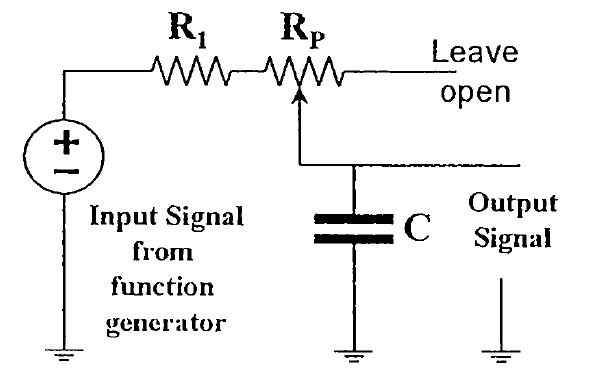
\includegraphics[width=0.8\linewidth]{1.jpg}
		\caption{First-Order Circuit.}
	\end{figure}
	The obtained data is presented in Table 1.
	\subsection{Second-Order Circuit}
	\begin{itemize}
		\item $L=1\rm{mH}$, $R_2=100\Omega$, $C=820\rm{pF}$;
		\item Steps:
		\begin{enumerate}[1.]
			\item On the function generator, set a square wave at 1$\rm{V_{ppk}}$ and 10 kHz as the input signal.
			\item Vary $R_P$ to generate three kinds of plot on the oscilloscope. (Under-damped, critically damped, over-damped response).
			\item Observe and save the graph from the oscilloscope.
			\item Record: Fall time and Rise time, the time interval between the neighboring peaks, $\Delta t$, and the resistance of the potentiometer, $R_P$.
		\end{enumerate}
	\end{itemize}
	\begin{figure}[H]
		\centering
		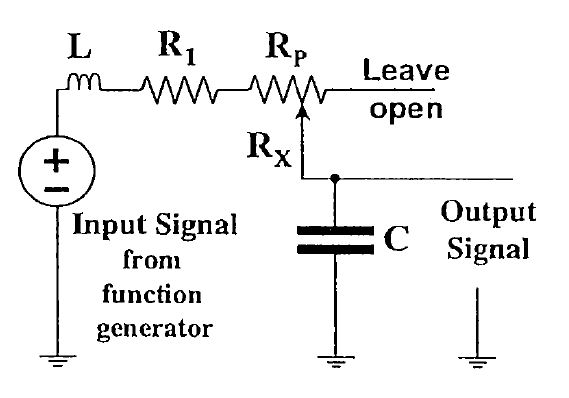
\includegraphics[width=0.8\linewidth]{2.jpg}
		\caption{First-Order Circuit.}
	\end{figure}
	The obtained data is presented in Table 2.
	\section{Results \& Calculations}
	\subsection{First-Order Circuit}
	\begin{table}[H]
		\centering
		\begin{tabular}{|c|>{\makecell*[c]}c|c|}
			\hline
			\makecell[l]{The setting of the potentiometer\\Corresponds to the …}&Fastest circuit response&Slowest circuit response\\
			\hline
			\makecell[l]{Peak to peak voltage of the\\Input square wave, $\rm{V_{ppk}}$ [V]}&2.000&2.000\\
			\hline
			\makecell[l]{Peak to peak voltage of the\\Output square wave, $\rm{V_{ppk}}$ [V]}&2.13&2.13\\
			\hline
			Period of the Input square wave, T [ms]&10.0000000&10.0000000\\
			\hline
			Rise Time of the Output waveform, [ms]&0.1738&1.6044\\
			\hline
			Fall Time of the Output waveform, [ms]&0.1920&1.7192\\
			\hline
		\end{tabular}
		\caption{First-Order Circuit.}
	\end{table}
	\begin{figure}[H]
		\centering
		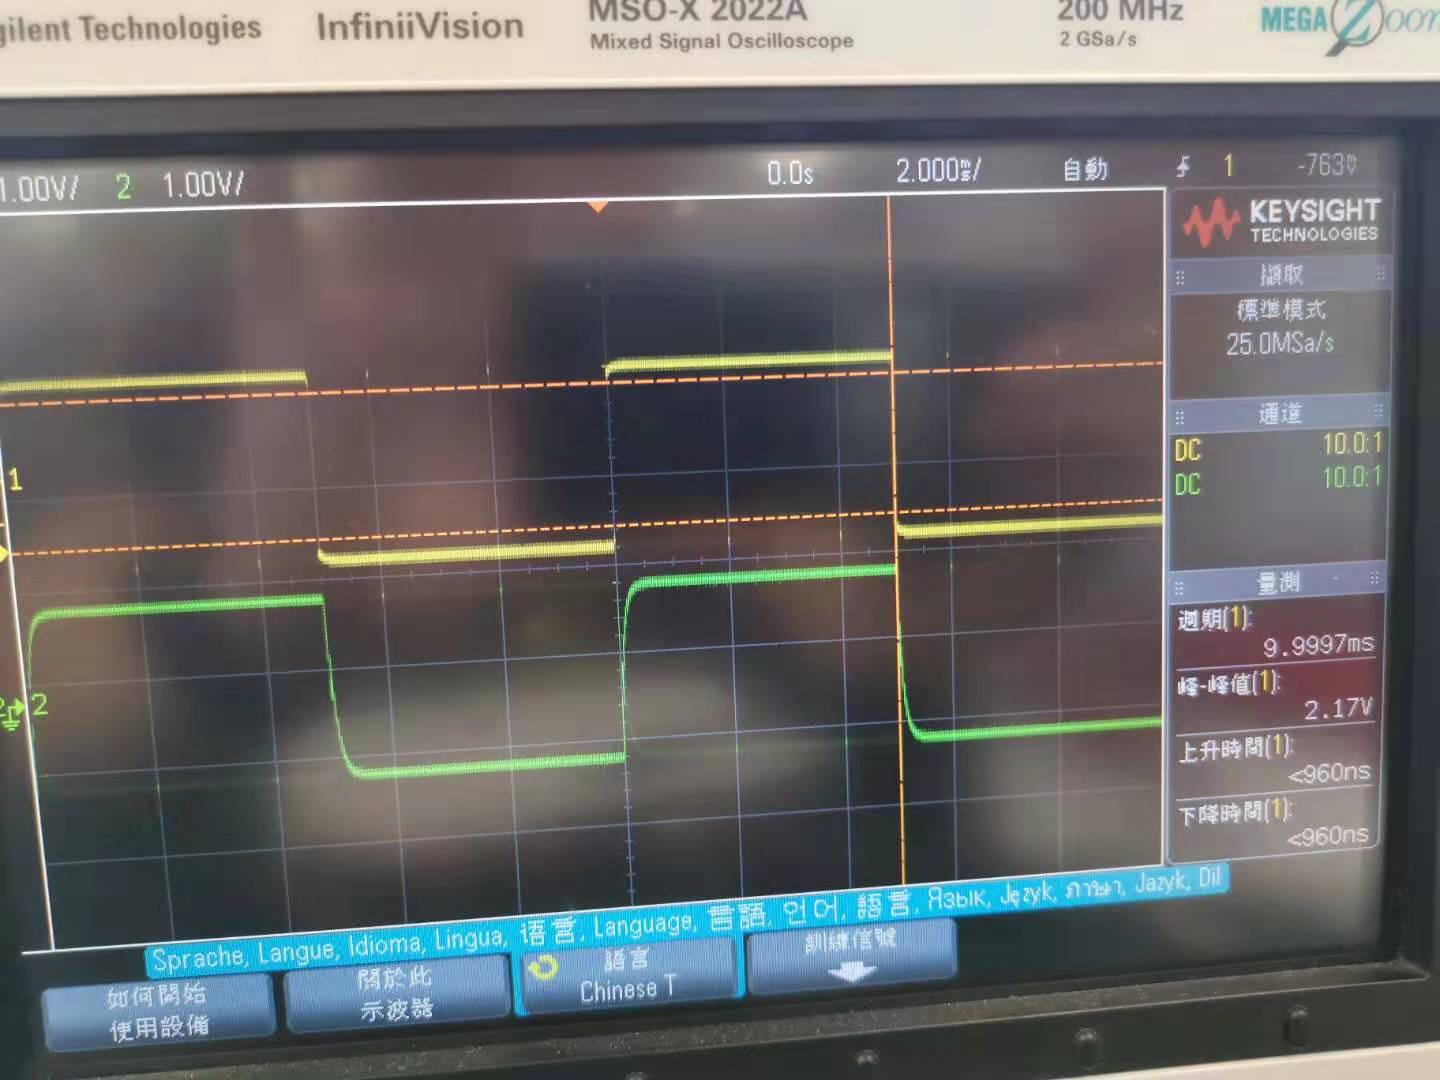
\includegraphics[width=0.8\linewidth]{3.jpg}
		\caption{First-Order Circuit.}
	\end{figure}
	\subsection{Second-Order Circuit}
	\begin{table}[H]
		\centering
		\begin{tabular}{|c|c|c|c|c|}
			\hline
			&Resistance $R_P$&Rise Time, [ms],&Fall Time, [ms]&time interval, $\Delta t$\\
			\hline
			\multirow{2}{*}{Under-damped}&484$\Omega$&0.001160&0.001164&0.005600000\\
			\cline{2-5}
			&301.4$\Omega$&0.001050&0.001070&0.005800000\\
			\hline
			critically damped&1989$\Omega$&0.002958&0.002816&\\
			\hline
			\multirow{2}{*}{over-damped}&3207$\Omega$&0.005268&0.004872&\\
			\cline{2-5}
			&4.57k$\Omega$&0.009286&0.008756&\\
			\hline
		\end{tabular}
		\caption{Second-Order Circuit.}
	\end{table}
	\begin{figure}[H]
		\centering
		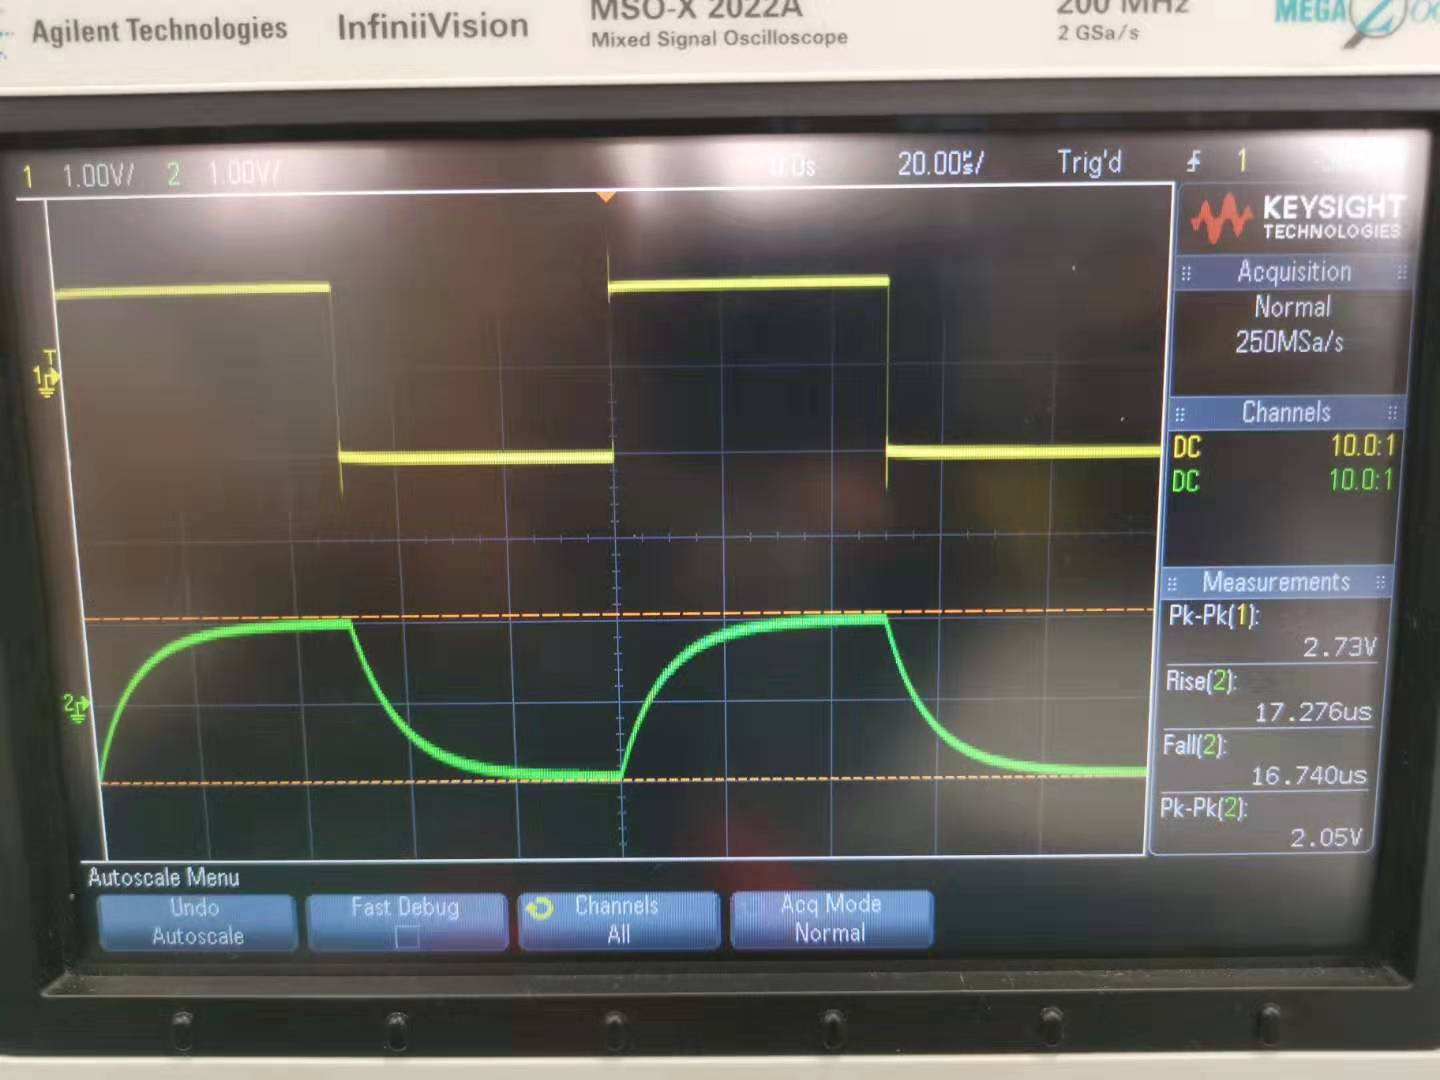
\includegraphics[width=0.8\linewidth]{4.jpg}
		\caption{First-Order Circuit Under-damped.}
	\end{figure}
	\begin{figure}[H]
		\centering
		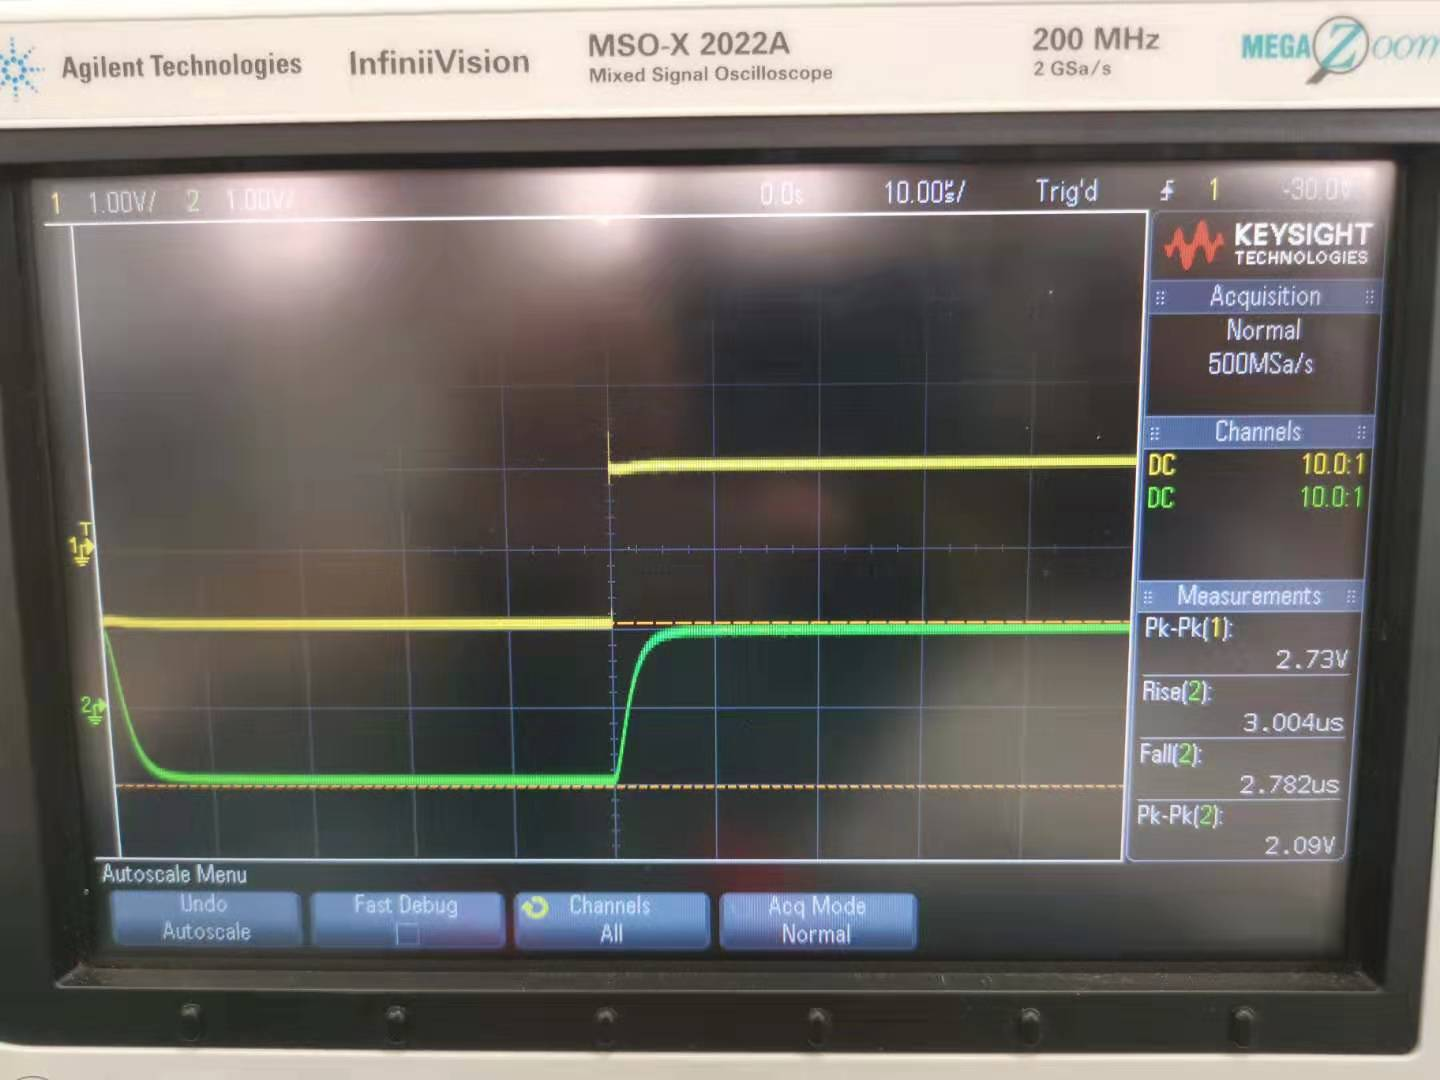
\includegraphics[width=0.8\linewidth]{5.jpg}
		\caption{First-Order Circuit Critically Damped.}
	\end{figure}
	\begin{figure}[H]
		\centering
		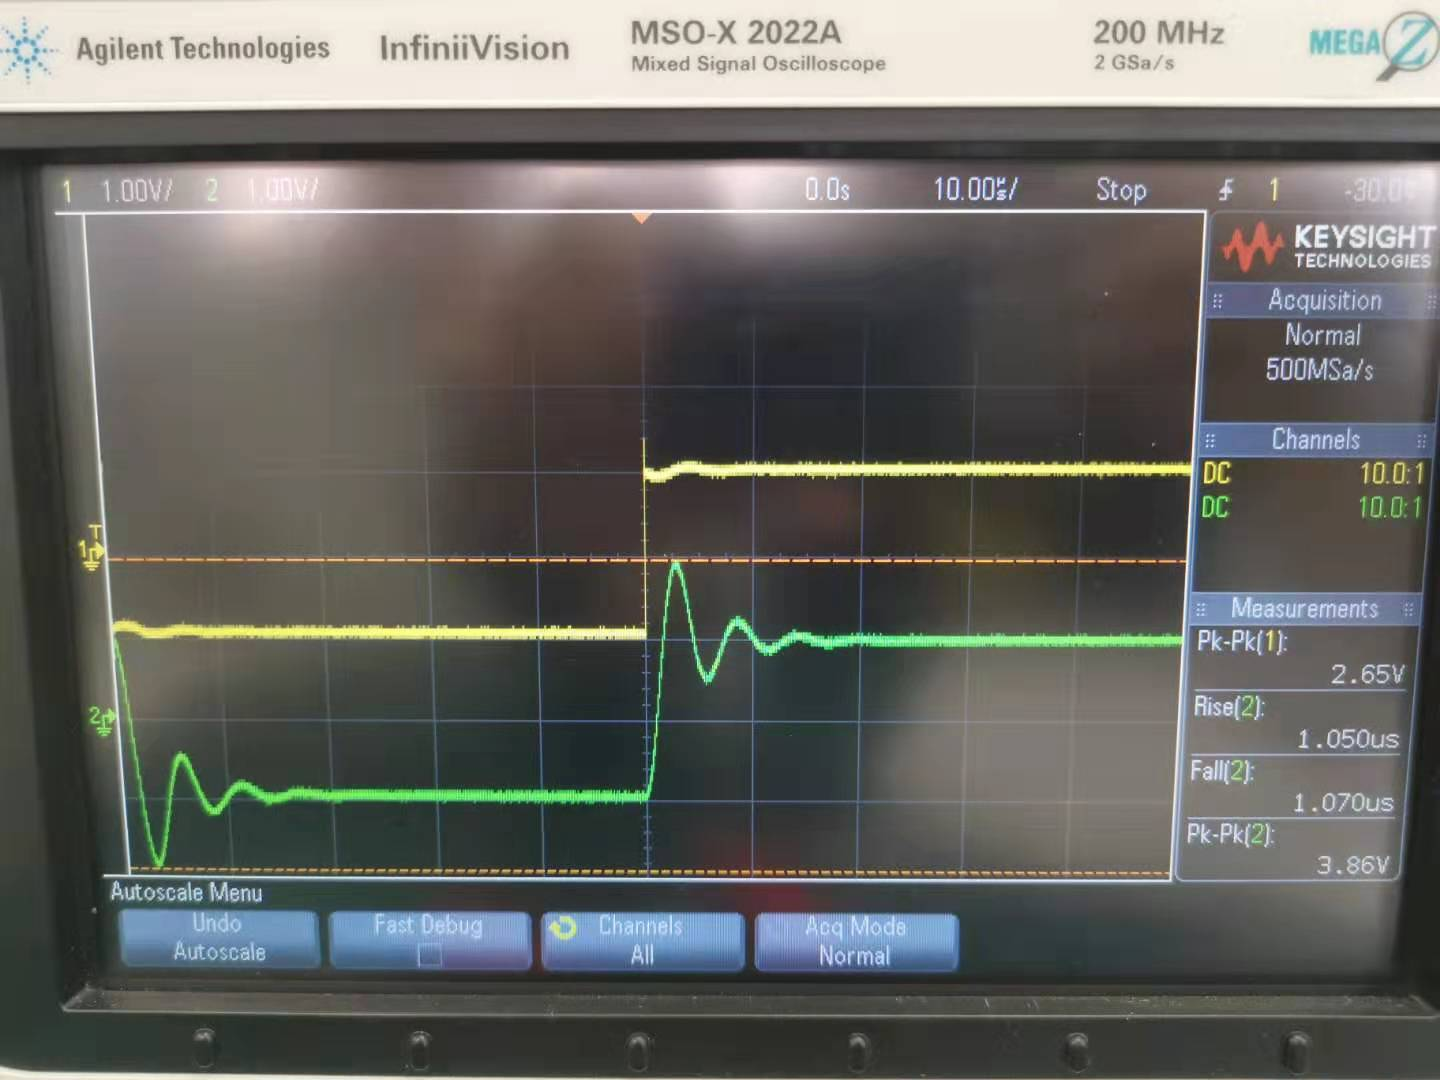
\includegraphics[width=0.8\linewidth]{6.jpg}
		\caption{First-Order Circuit Over-damped.}
	\end{figure}
	\section{Conclusions and Discussion}
	In this experiment, we succeeded to build a series $RC$ and a $RLC$ circuit and observe their responses to variable input square wave signal. We adjusted the oscilloscope and measured the peak-to-peak voltage, the period, the rise time of the input square wave, and the fall time of the output waveform, from where we learned the step responses in first and second order circuits.
	
	When we firstly built our $RC$ circuit and tried to obtained an ideal waveform, the waveform on the oscilloscope is not measurable. The observed rise time and fall time were so short that the waveform was quite weak as we used smaller and smaller scale, so we used another machine to continue our experiment. Although it seemed that the rise time and the fall time are quite short, we were told that they were large enough, and eventually it turned out that they were reasonable. By adjusting the variable resistor, we changed the responses of the $RLC$ circuit and the waveforms on the oscilloscope corresponds to the theoretical graphs.
	
	Last but not least, we build the $LC$ tank and make observation in short. I think it is important to check whether a machine is working properly.
	\vspace{3cm}
	\section*{Data Sheet}
\end{document}